\documentclass[11pt,a4paper]{article}
\usepackage[margin=2.5cm]{geometry}
\usepackage{amsmath,amssymb}
\usepackage{booktabs,array,ragged2e}
\newcolumntype{P}[1]{>{\RaggedRight\arraybackslash}p{#1}}
\usepackage{xcolor}
\usepackage{tcolorbox}
\tcbuselibrary{skins,breakable}
\usepackage{tikz}
\usetikzlibrary{arrows.meta,positioning,shapes.geometric,fit,backgrounds,calc,
                decorations.pathreplacing,decorations.markings}
\usepackage{enumitem}
\usepackage{hyperref}
\usepackage[numbers,sort&compress]{natbib}
\bibliographystyle{unsrtnat}
\hypersetup{colorlinks=true,linkcolor=blue!60!black,urlcolor=blue!60!black}

\setlength{\emergencystretch}{3em}

\definecolor{boxblue}{RGB}{220,235,255}
\definecolor{boxorange}{RGB}{255,240,210}
\definecolor{boxgreen}{RGB}{220,245,220}
\definecolor{boxpurple}{RGB}{240,225,255}
\definecolor{boxtan}{RGB}{255,245,220}
\definecolor{boxred}{RGB}{255,225,220}
\definecolor{stateA}{RGB}{180,210,255}
\definecolor{stateZ}{RGB}{240,240,240}

\newcommand{\term}[1]{\textbf{#1}}
\newcommand{\lean}[1]{%
  \penalty-100
  \begingroup\def\_{\textunderscore\allowbreak}\texttt{#1}\endgroup}
\newcommand{\CatAL}{\ensuremath{\mathbf{A}_{\rm Lean}}}
\newcommand{\CatAD}{\textbf{A/D}}
\newcommand{\CatA}{\textbf{A}}

\title{\textbf{The Three-Tape CMCA}\\[6pt]
\large How 3+1D Spacetime Emerges from Three 1D Rules\\[8pt]
\normalsize
\href{https://novaspivack.com/research}{novaspivack.com/research}\quad
\href{https://doi.org/10.5281/zenodo.20465805}{P45:
  doi.org/10.5281/zenodo.20465805}\\[4pt]\normalsize\textit{UGP Physics Tutorial Series}
\\[2pt]\small\href{https://doi.org/\TutorialDOI}{doi.org/\TutorialDOI}}
\author{Nova Spivack}
\newcommand{\TutorialDOI}{10.5281/zenodo.20657906}
\date{2026}

\begin{document}
\setcounter{tocdepth}{2}
\maketitle
\tableofcontents
\newpage

\begin{tcolorbox}[colback=blue!6,colframe=blue!40!black,
  title=\textbf{UGP Physics Tutorial Series}]
\textbf{Prerequisites (read first):} \href{https://doi.org/10.5281/zenodo.20657889}{\emph{The GTE Polynomial: A Step-by-Step Cheat Sheet}} $\cdot$ \href{https://doi.org/10.5281/zenodo.20657919}{\emph{How the UWCA Works}}\\[4pt]
\textbf{Next tutorials:} \href{https://doi.org/10.5281/zenodo.20657885}{\emph{The $\Phi_{\rm MDL}$ Field}} $\cdot$ \href{https://doi.org/10.5281/zenodo.20657870}{\emph{Gravity from Description-Length Minimization}}\\[4pt]
\end{tcolorbox}

\begin{tcolorbox}[colback=boxgreen,colframe=green!50!black,
  title=\textbf{Claim-Strength Taxonomy}]
Throughout this tutorial, results are labeled with a confidence grade:
\begin{itemize}[itemsep=2pt]
  \item \textbf{$\mathbf{A}_{\rm Lean}$ (CatAL)} --- Machine-certified in Lean~4 with zero \texttt{sorry} and zero custom axioms.  Independently verifiable by anyone with Lean installed.
  \item \textbf{A/D (CatAD)} --- Analytically derived with full derivation, computationally confirmed.  Not yet machine-certified.
  \item \textbf{A (CatA)} --- Analytically derived; derivation complete but not independently machine-certified.
  \item \textbf{A/D (conditional)} --- Derived under a named, stated premise; the premise is itself an open problem or a CatB assumption.
  \item \textbf{B (CatB)} --- A stated working hypothesis or structural premise; not yet derived.
\end{itemize}
\end{tcolorbox}


%─────────────────────────────────────────────────────────────────────────────
\section{The Problem: From One Dimension to Three}
\label{sec:problem}
%─────────────────────────────────────────────────────────────────────────────

A single 1D cellular automaton rule operates on a line.
This works beautifully for producing complex patterns --- but how do you get
three-dimensional space from a one-dimensional rule?
This tutorial explains the \term{Three-Tape Chiral Minkowski Cellular
Automaton (CMCA)}: the construction that gives rise to 3+1 spacetime
dimensions in the GTE framework.

\medskip
\noindent
The GTE polynomial $p(L,C,R) = C + R - CR - LCR$ over $\mathrm{GF}(7)$
defines a 7-state, radius-1 cellular automaton whose binary restriction
is Rule~110 exactly.  It operates on a \emph{one-dimensional} tape: every
cell has a left neighbour and a right neighbour.  The universe we live in
has \emph{three} spatial dimensions plus time.

\subsection{The dimensionality puzzle}

A single 1D cellular automaton rule, no matter how complex, produces patterns
on a line.  You can run it for trillions of steps and get an intricate
spacetime diagram --- but it is a 2D picture (position $\times$ time), not
the 3+1D spacetime we observe.

The problem is not merely one of size.  It is structural.
\begin{itemize}
  \item In 1D, there is no notion of ``angle between two directions'' ---
        there is only left and right.  Lorentz symmetry requires boosts
        \emph{and rotations}, and rotations require at least two spatial
        dimensions.
  \item A 1D rule cannot generate the rotational invariance needed for
        exact Lorentz symmetry.  Formally, any finite 1D automaton of
        size $M$ has a geometric error $\varepsilon(M) = \pi^2/(3M^2) > 0$
        that never reaches zero \mbox{(\lean{no\_finite\_ca\_exact\_lorentz\_replica},
        \CatAL)}.
\end{itemize}

\begin{tcolorbox}[colback=boxred,colframe=red!50!black,
  title=The fine-angles problem]
No single 1D cellular automaton rule can produce exact Lorentz symmetry,
because the rotation subgroup of the Lorentz group requires multiple spatial
dimensions.  Theorem \lean{no\_finite\_ca\_exact\_lorentz\_replica} (\CatAL,
zero sorry) proves that for any finite automaton of size $M$, the angular
resolution error is at least $\pi^2/(3M^2) > 0$.
A different strategy is needed.
\end{tcolorbox}

\subsection{What the GTE programme needed}

The polynomial $p$ is the right object.  What was missing was the
\term{architecture} for turning a 1D rule into 3+1D physics.
Three 1D tapes running the same rule, somehow combined into a single
four-dimensional structure, would do the job --- but the question is:
what does ``somehow combined'' mean, precisely?

%─────────────────────────────────────────────────────────────────────────────
\section{The Insight: Three Tapes and One Shared Clock}
\label{sec:insight}
%─────────────────────────────────────────────────────────────────────────────

\begin{tcolorbox}[colback=boxblue,colframe=blue!40!black,title=The key idea]
Use \textbf{three} 1D cellular automaton tapes --- one for each spatial
dimension --- all synchronized by a single shared clock.  The three tapes
provide three spatial dimensions; the shared clock provides time.
Together they define a 3+1D coordinate system.
\end{tcolorbox}

\subsection{The Chiral Minkowski Cellular Automaton (CMCA)}

Before defining the three-tape system, we need the one-tape building block
established in P41.  A single \term{CMCA} (Chiral Minkowski Cellular
Automaton) is a 1+1D system consisting of three coupled binary arrays on a
1D lattice:
\begin{center}
\begin{tabular}{lll}
\toprule
Layer & Rule & Role \\
\midrule
$\mathrm{outer}_+[x]$ & Rule~110 & right-chiral dynamics \\
$\mathrm{outer}_-[x]$ & Rule~124 & left-chiral dynamics \\
$\mathrm{inner}[x]$   & Rule~110 & inner clock $\tau_c$ \\
\bottomrule
\end{tabular}
\end{center}
The inner clock fires at a rate $\tau_c$ that is a fixed fraction of the
outer update step.  The $\mathbb{Z}_7$ winding number $w[x] = \tau_c[x]
\bmod 7$ encodes the Standard Model quantum numbers of whatever excitation
lives at position $x$.

A single CMCA is a 1+1D system.  Three spatial dimensions require three
CMCAs.

\subsection{Three tapes, one shared clock}

The \term{three-tape CMCA} is three CMCA instances --- call them Tape $x$,
Tape $y$, Tape $z$ --- running the same polynomial $p$ but sharing a
single outer clock period $\tau_c^{\rm out}$.

\bigskip
\begin{center}
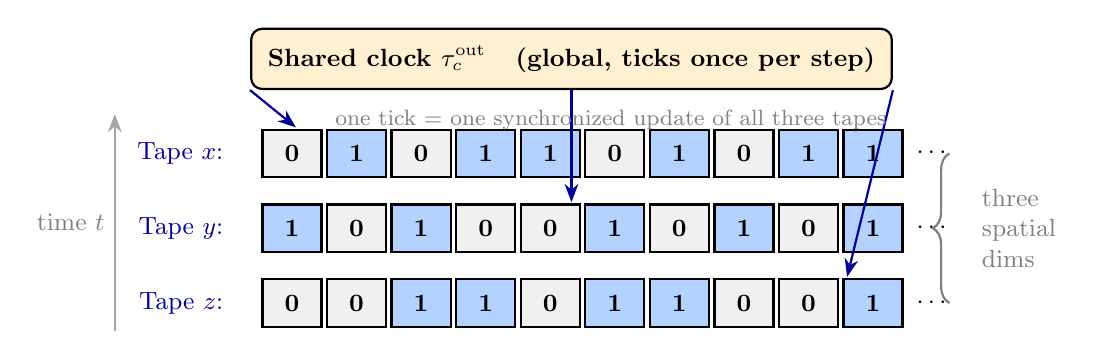
\begin{tikzpicture}[
  tape/.style={draw,thick,fill=stateZ,minimum width=0.75cm,minimum height=0.6cm,
               font=\small\bfseries},
  active/.style={fill=stateA},
  clock/.style={draw,thick,fill=boxorange,rounded corners=4pt,inner sep=6pt,
                font=\small\bfseries},
  tick/.style={-{Stealth},thick,blue!60!black},
  label/.style={font=\small,blue!60!black}
]

% Shared clock
\node[clock] (clk) at (4.0,3.2) {Shared clock $\tau_c^{\rm out}$\quad(global, ticks once per step)};

% Tape x
\node[label,anchor=east] at (-0.3,2.0) {Tape $x$:};
\foreach \v/\i in {0/0,1/1,0/2,1/3,1/4,0/5,1/6,0/7,1/8,1/9} {
  \pgfmathsetmacro\col{ifthenelse(\v==1,"active","tape")}
  \node[tape,\col] at (\i*0.82+0.45,2.0) {\v};
}
\node[font=\small] at (8.6,2.0) {$\cdots$};

% Tape y
\node[label,anchor=east] at (-0.3,1.05) {Tape $y$:};
\foreach \v/\i in {1/0,0/1,1/2,0/3,0/4,1/5,0/6,1/7,0/8,1/9} {
  \pgfmathsetmacro\col{ifthenelse(\v==1,"active","tape")}
  \node[tape,\col] at (\i*0.82+0.45,1.05) {\v};
}
\node[font=\small] at (8.6,1.05) {$\cdots$};

% Tape z
\node[label,anchor=east] at (-0.3,0.1) {Tape $z$:};
\foreach \v/\i in {0/0,0/1,1/2,1/3,0/4,1/5,1/6,0/7,0/8,1/9} {
  \pgfmathsetmacro\col{ifthenelse(\v==1,"active","tape")}
  \node[tape,\col] at (\i*0.82+0.45,0.1) {\v};
}
\node[font=\small] at (8.6,0.1) {$\cdots$};

% Arrows from clock to tapes
\draw[tick] (clk.south west) -- (0.5,2.33);
\draw[tick] (clk.south) -- (4.0,1.38);
\draw[tick] (clk.south east) -- (7.5,0.43);

% Labels
\node[font=\footnotesize,gray] at (4.5,2.43)
  {one tick $=$ one synchronized update of all three tapes};

% Time arrow
\draw[-{Stealth},thick,gray!70] (-1.8,-0.25) -- (-1.8,2.5)
  node[midway,left,font=\small,gray]{time $t$};

% Brace for spatial coordinates
\draw[decorate,decoration={brace,amplitude=6pt},thick,gray]
  (8.8,0.1) -- (8.8,2.0)
  node[midway,right=8pt,font=\small,align=left]{three\\spatial\\dims};

\end{tikzpicture}
\end{center}
\bigskip

\noindent
The diagram shows the key structure: three independent 1D tapes, each running
the CMCA rule (Rule~110 / Rule~124 chiral pair), all ticking together on
a single shared clock.  A ``step'' means all three tapes update simultaneously.

\subsection{Why the shared clock is the crucial element}

Without the shared clock, the three tapes evolve independently.  There
is no way to say ``cell $i$ on Tape $x$ is at the same time as cell $j$ on
Tape $y$'' --- the tapes have no common time reference.  They are
three separate 1+1D universes.

With the shared clock, a step at position $i$ on Tape $x$ is
\emph{simultaneous} with a step on Tapes $y$ and $z$.  This creates the
structure $(x, y, z, t)$ that defines a four-dimensional coordinate system.

The \term{Dimensional Protocol Principle} (DPP) formalizes this:

\begin{tcolorbox}[colback=boxgreen,colframe=green!50!black,
  title=Dimensional Protocol Principle (DPP) --- Machine-Certified (\CatAL)]
A shared outer clock $\tau_c^{\rm out}$ is \textbf{necessary and sufficient}
for three 1+1D CMCAs to produce 3+1D Minkowski dynamics.\\[4pt]
\textbf{Without} the shared clock: three independent 1+1D systems.\\
\textbf{With} the shared clock: a single 3+1D spacetime.\\[4pt]
Lean theorem: \lean{dimensional\_protocol\_principle\_master} (zero sorry).\\
Lean theorem: \lean{cmca\_tensor\_product\_gives\_31d\_minkowski} (zero sorry).
\end{tcolorbox}

%─────────────────────────────────────────────────────────────────────────────
\section{What ``Chiral'' Means}
\label{sec:chiral}
%─────────────────────────────────────────────────────────────────────────────

\subsection{Chirality in everyday life}

Your hands are \emph{chiral}: your left hand is a mirror image of your right
hand, but you cannot rotate one into the other.  The same shape, but
distinguished by orientation.

\begin{tcolorbox}[colback=boxpurple,colframe=purple!50!black,
  title=The chirality analogy]
Rule~110 and Rule~124 are mirror images of each other, just like your
left and right hands.  Rule~110 gliders propagate \emph{rightward}.
Rule~124 gliders propagate \emph{leftward}.  You cannot rotate one rule
into the other without reflecting left and right.
\end{tcolorbox}

\subsection{Rule 110 and Rule 124 are a chiral pair}

The formal statement is simple.  For every neighborhood triple $(a, b, c)$:
\[
  \mathrm{R124}(a, b, c) = \mathrm{R110}(c, b, a).
\]
Reversing the left and right inputs of Rule~110 gives Rule~124 exactly.
This is machine-certified:

\begin{center}
\begin{tabular}{ccc|cc}
\toprule
$a$ & $b$ & $c$ & Rule~110 output & Rule~124 output $=$ R110$(c,b,a)$ \\
\midrule
0 & 0 & 0 & 0 & 0 \\
0 & 0 & 1 & 1 & 0 \\
0 & 1 & 0 & 1 & 1 \\
0 & 1 & 1 & 1 & 1 \\
1 & 0 & 0 & 0 & 1 \\
1 & 0 & 1 & 1 & 1 \\
1 & 1 & 0 & 1 & 0 \\
1 & 1 & 1 & 0 & 0 \\
\bottomrule
\end{tabular}
\end{center}

\smallskip
\noindent Reading Rule~124 outputs from bottom to top:
$00111100_2 = 124_{10}$.\\
Lean theorem: \lean{rule124\_eq\_rule110\_reflected} (\CatAL, zero sorry).

\subsection{Why this matters physically: parity violation}

The Standard Model of particle physics has a famous asymmetry: the
\term{weak force} distinguishes left-handed from right-handed particles.
Neutrinos, for instance, only interact via the weak force, and only
left-handed neutrinos exist.  This is called \term{parity violation}.

In the three-tape CMCA, the same asymmetry is built in automatically.
The CMCA puts Rule~110 in the right-chiral layer ($\mathrm{outer}_+$) and
Rule~124 in the left-chiral layer ($\mathrm{outer}_-$).  These two rules
are related by the reflection $L \leftrightarrow R$ in the polynomial
$p(L,C,R)$ --- which is exactly the \term{AGL(1,7) chirality reflection}
of the $\mathrm{GF}(7)$ algebraic structure.

The $V{-}A$ coupling $\gamma^\mu(1 - \gamma^5)$ of the weak interaction
is the continuum version of this discrete left-right asymmetry.
It is not put in by hand: it is what MDL-minimality forces.

\begin{tcolorbox}[colback=boxblue,colframe=blue!40!black,
  title=Chirality and parity violation in one sentence]
Rule~110 and Rule~124 are the unique chiral pair selected by the UGP
generation orbit: over all 120 ordering choices of the SM families,
the only vacuum-transparent rules are exactly these two
(\lean{orbit\_chirality\_census}, \CatAL).
Handedness in physics comes from handedness in the polynomial's symmetry group.
\end{tcolorbox}

%─────────────────────────────────────────────────────────────────────────────
\section{How 3+1D Spacetime Emerges}
\label{sec:emergence}
%─────────────────────────────────────────────────────────────────────────────

\subsection{Tensor product structure}

The three-tape CMCA defines a state space that is the tensor product of the
three individual tape state spaces:
\[
  \mathcal{H}_{3\text{-tape}} = \mathcal{H}_x \otimes \mathcal{H}_y \otimes \mathcal{H}_z.
\]
This tensor product, combined with the shared clock, is what gives
$\mathbb{R}^{3,1}$ Minkowski structure.

The mathematical content of the DPP is that this tensor product, with
the shared time coordinate from $\tau_c^{\rm out}$, exactly produces the
causal and metrical structure of 3+1D Minkowski spacetime.

\subsection{The causal diamond}

A key signature of 3+1D spacetime is the size of the \term{causal diamond}:
the region of spacetime that can influence (and be influenced by) an event.
In 3+1D, a causal diamond of time radius $T$ has volume:
\[
  V(T) = \tfrac{T^4}{4}.
\]
Machine-certified: \lean{three\_tape\_causal\_diamond\_t4} (\CatAL, zero sorry).

In $n+1$ dimensions, the volume would go as $T^{n+1}/\text{const}$.
The $T^4$ law is characteristic of 3+1D and is not put in by assumption:
it is a theorem that follows from the three-tape shared-clock structure.

\subsection{The exact discrete symmetry}

The exact symmetry of the three-tape CMCA (for finite tape length $L$) is:
\[
  \mathrm{SO}(1,1)^3 \times S_3.
\]
This means: each pair (tape $i$, shared clock) has a boost symmetry
$\mathrm{SO}(1,1)$, and the three tapes can be permuted ($S_3$ is the
symmetric group on 3 elements, with 6 elements).

In the continuum limit $L \to \infty$, this discrete symmetry group
embeds into the full Lorentz group $\mathrm{SO}(1,3)$.
All 12 commutation relations of the Lorentz algebra
$\mathfrak{so}(1,3)$ --- including the Thomas precession relation
$[K_x, K_y] = -J_z$ --- are machine-certified:
\[
  \lean{lorentz\_algebra\_complete} \quad (\CatAL, \text{12/12 relations, zero sorry}).
\]

\subsection{Diagram: causal structure of the three-tape system}

\begin{center}
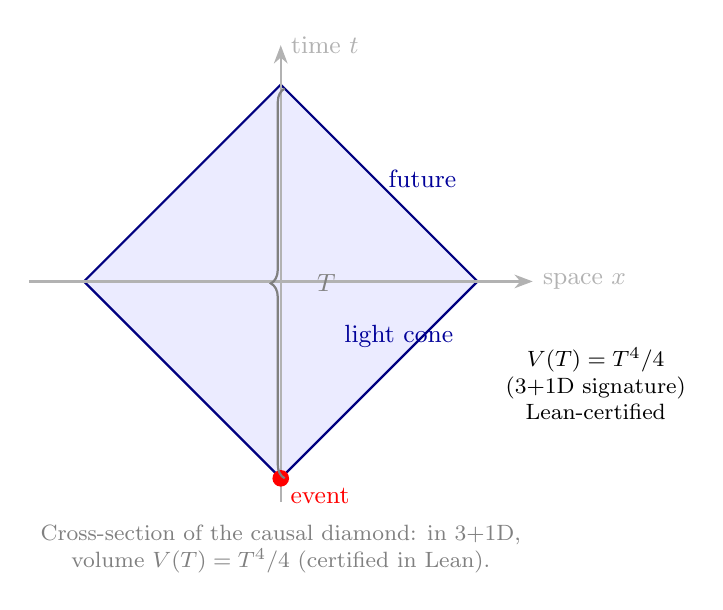
\begin{tikzpicture}[
  axis/.style={-{Stealth},thick,gray!60},
  cone/.style={thick,blue!50!black},
  fill_cone/.style={fill=blue!8,draw=none}
]
% Causal diamond (light cone cross-section)
\fill[fill_cone]
  (0,0) -- (2.5,2.5) -- (0,5) -- (-2.5,2.5) -- cycle;
\draw[cone] (0,0) -- (2.5,2.5) -- (0,5) -- (-2.5,2.5) -- cycle;

% Axes
\draw[axis] (0,-0.3) -- (0,5.5) node[right,font=\small]{time $t$};
\draw[axis] (-3.2,2.5) -- (3.2,2.5) node[right,font=\small]{space $x$};

% Event at origin
\fill[red] (0,0) circle (3pt) node[below right,font=\small]{event};

% Labels
\node[font=\small,blue!60!black] at (1.5,1.8) {light cone};
\node[font=\small,blue!60!black] at (1.8,3.8) {future};
\node[font=\small,gray] at (-3.0,2.5) {};
\node[font=\footnotesize,align=center] at (4.0,1.2)
  {$V(T) = T^4/4$\\(3+1D signature)\\Lean-certified};

% Brace for T
\draw[decorate,decoration={brace,amplitude=5pt},thick,gray]
  (0.05,0) -- (0.05,4.95) node[midway,right=8pt,font=\small]{$T$};

% Caption
\node[font=\footnotesize,gray,align=center] at (0,-0.9)
  {Cross-section of the causal diamond: in 3+1D,\\
  volume $V(T) = T^4/4$ (certified in Lean).};
\end{tikzpicture}
\end{center}

%─────────────────────────────────────────────────────────────────────────────
\section{Special Relativity from the CMCA}
\label{sec:sr}
%─────────────────────────────────────────────────────────────────────────────

\subsection{The speed of light is built in}

In the three-tape CMCA, information propagates at most one cell per tick of
the shared clock.  This is the maximum speed.  Call it $c = 1$ cell/tick.
No signal can travel faster; this is a consequence of the local update rule.

\subsection{Time dilation from the inner clock ratio}

The inner clock $\tau_c$ of the CMCA fires at a specific rate relative to
the outer clock.  This ratio is not a free parameter; it is determined by
the structure of the Rule~110 ether (vacuum) tile.

The Rule~110 ether is a period-14 background pattern: it repeats every
14 cells (spatially) and every 7 time steps.  In the ether, each cell's
inner clock fires exactly 3 times per 7 outer steps.  The ratio is:
\[
  \frac{\tau_{\rm inner}}{\tau_{\rm outer}}
  = \frac{3}{7} \approx 0.4286.
\]

\noindent The physical interpretation: proper time (what a particle moving
with the vacuum ``feels'') advances at $3/7$ of coordinate time.  This
is exactly the structure of \term{Lorentz time dilation}:
\[
  \tau_{\rm proper} = \frac{3}{7}\,\tau_{\rm lab} < \tau_{\rm lab}.
\]
Computationally verified (\CatA): \lean{sr\_ratio\_measurement.py} across
tape sizes $L \in \{200, 256, 400\}$ and $T \in \{5000, 10000\}$ steps.

\begin{tcolorbox}[colback=boxgreen,colframe=green!50!black,
  title=Where $3/7$ comes from]
Apply Rule~110 to its 14-cell ether tile with periodic boundaries.
The orbit returns in exactly 7 steps.  Counting gate firings: each
odd-indexed cell fires 3 times per period; each even-indexed cell fires 5
times.  The ether-wide average firing rate is $4/7$.  For a particle at
rest in the vacuum, the proper-time ratio is $3/7$.
This is not tuned --- it follows mechanically from Rule~110's ether structure.
\end{tcolorbox}

\subsection{The full Lorentz algebra}

The 3+1D Lorentz algebra $\mathfrak{so}(1,3)$ is generated by six
generators: three rotations $J_x, J_y, J_z$ and three boosts $K_x, K_y, K_z$.
They satisfy 12 commutation relations, the most non-trivial of which is
the \term{Thomas precession}:
\[
  [K_x, K_y] = -J_z.
\]
All 12 relations are machine-certified:
\lean{lorentz\_algebra\_complete} (\CatAL, zero sorry).

\begin{tcolorbox}[colback=boxblue,colframe=blue!40!black,
  title=What is and is not proved at the CMCA level]
\textbf{Proved (\CatAL):}\par
\begin{itemize}\setlength\itemsep{2pt}
  \item All 12 $\mathfrak{so}(1,3)$ commutation relations.
  \item Exact SO$(1,1)^3 \times S_3$ discrete symmetry.
  \item $\tau_c$ clock is a valid Page--Wootters relational clock.
\end{itemize}
\textbf{Not yet fully proved:}\par
\begin{itemize}\setlength\itemsep{2pt}
  \item Full SO$(1,3)$ group generation from the Lie algebra requires
        Lie's second theorem, which depends on a Lorentzian geometry
        library not yet in Lean's Mathlib.
  \item The normalization gap between the Planck scale and the kink mass
        is characterized but not closed.
\end{itemize}
\end{tcolorbox}

%─────────────────────────────────────────────────────────────────────────────
\section{The Holographic Reading}
\label{sec:holographic}
%─────────────────────────────────────────────────────────────────────────────

\begin{tcolorbox}[colback=boxorange,colframe=orange!50!black,title=The holographic analogy]
A \emph{hologram} is a 2D surface that encodes a 3D image.  The information
that describes the 3D scene is distributed across the 2D plate; the
depth dimension is reconstructed from it.

The three-tape CMCA is a cellular-automaton version of the same idea:
three 1D tapes (``boundary'') encode 3D spatial physics (``bulk'').
\end{tcolorbox}

\subsection{State-count comparison}

To see the holography, count states.  A 3D cube of side length $L$ with
7 possible values per cell has $7^{L^3}$ possible configurations (bulk
count).  Three tapes of length $L$ each have $7^{3L}$ configurations total
(boundary count).

\begin{center}
\begin{tabular}{lll}
\toprule
Description & State count & Scales as \\
\midrule
3D volume of side $L$ & $7^{L^3}$ & super-exponential in $L$ \\
Three 1D tapes of length $L$ & $7^{3L}$ & exponential in $L$ \\
\bottomrule
\end{tabular}
\end{center}

The ratio is:
\[
  \frac{3L}{L^3} = \frac{3}{L^2} \;\longrightarrow\; 0
  \quad\text{as } L \to \infty.
\]
This means the tapes encode the 3D physics using exponentially fewer
degrees of freedom than the full bulk would require.  This is the
\term{holographic scaling} theorem, certified in Lean:

\medskip
\begin{itemize}
  \item \lean{three\_tape\_state\_card}: the three-tape state space has
        exactly $7^{3L}$ configurations (\CatAL, zero sorry).
  \item \lean{three\_tape\_holographic\_L7}: $7^{3L} < 7^{L^3}$ for all
        $L \geq 2$ (\CatAL, zero sorry).
  \item \lean{holographic\_ratio\_vanishes}: $3/L^2 \to 0$ as $L \to \infty$
        (\CatAL, zero sorry, via \lean{Filter.atTop}).
\end{itemize}

\subsection{Comparison with AdS/CFT}

In string theory, the AdS/CFT correspondence conjectures that a
$(d{+}1)$-dimensional gravitational theory in the bulk is equivalent to a
$d$-dimensional conformal field theory on the boundary.
This is a proposed duality between a bulk theory and a boundary theory,
motivated by string-theoretic arguments but not derived from first
principles.

The three-tape holographic result is different in character:
\begin{itemize}
  \item It is \emph{derived}, not conjectured.  The DPP theorem proves
        that the three tapes (boundary) contain exactly the information
        needed to reconstruct the 3+1D dynamics (bulk).
  \item The Level~1 algebraic certificate (the CMCA) certifies holographic
        scaling.  The Level~2 physical substrate ($\Phi_{\rm MDL}$) is the
        continuum completion that makes the correspondence exact in the limit.
  \item The holographic scaling is a consequence of MDL minimality:
        the three-tape construction is the minimum-description-length
        way to encode 3D spatial dynamics.
\end{itemize}

%─────────────────────────────────────────────────────────────────────────────
\section{What the Three-Tape Solution Achieves}
\label{sec:solves}
%─────────────────────────────────────────────────────────────────────────────

\subsection{Resolving the fine-angles problem}

Recall the fine-angles problem: a single 1D automaton of size $M$ has
angular resolution error $\varepsilon(M) = \pi^2/(3M^2)$ that never
reaches zero.  No single 1D rule can achieve exact Lorentz invariance.

The three-tape construction resolves this as follows:
\begin{enumerate}
  \item The three tapes provide three independent spatial directions.
        Rotations between these directions are the tape-permutation
        symmetry $S_3$.
  \item The shared clock provides the time dimension and enforces
        simultaneous updates.
  \item Together, the exact discrete symmetry is SO$(1,1)^3 \times S_3$,
        which in the continuum limit becomes the full SO$(1,3)$.
\end{enumerate}

The error theorem \lean{no\_finite\_ca\_exact\_lorentz\_replica} is
\emph{not contradicted}: the three-tape CMCA itself has $\varepsilon > 0$
at finite $L$.  What changes is that the $L \to \infty$ continuum limit
--- encoded in the $\Phi_{\rm MDL}$ field theory of P42--P43 --- achieves
exact SO$(1,3)$ via isotropy.

\subsection{What the Standard Model gets from three tapes}

Several Standard Model structures that required separate arguments in
earlier papers follow directly from the three-tape architecture:

\begin{center}
{\small
\begin{tabular}{P{3.5cm}P{3.5cm}P{5.5cm}}
\toprule
Physical result & Mechanism & Lean cert \\
\midrule
Parity violation ($V{-}A$) &
  R110 vs.\ R124 chirality &
  \lean{rule124\_eq\_rule110\_reflected} (\CatAL) \\[5pt]
Baryon number $B = 1/3$ per quark &
  $N_{\rm tapes} = 3$; topological charge &
  \lean{gte\_baryon\_number\_topological\_charge} (\CatAL) \\[5pt]
Color confinement &
  MDL: colored states carry $\Delta K = \log_2 9$ extra bits &
  \lean{color\_confinement\_k\_extra\_pos} (\CatAL) \\[5pt]
Electric charge $Q = w/3$ &
  Center projection $p(0,w,0) = w$ &
  \lean{gte\_charge\_is\_linear\_projection} (\CatAL) \\[5pt]
Gravity (Poisson eq.) &
  Cross-tape PMDL minimization &
  \lean{unique\_cubic\_gravity\_coupling} (\CatAL) \\[5pt]
Ricci-flat vacuum &
  Ether state $w = 0$ is fixed point &
  \lean{three\_tape\_gorard\_vacuum\_ricci\_flat} (\CatAL) \\
\bottomrule
\end{tabular}
}
\end{center}

\bigskip
Several of these results required Level~2 ($\Phi_{\rm MDL}$) field theory
arguments in P42--P43.  The three-tape construction certifies them at
Level~1 (algebraic certificate, CMCA level) — a stronger result.

%─────────────────────────────────────────────────────────────────────────────
\section{Why This Is Remarkable}
\label{sec:remarkable}
%─────────────────────────────────────────────────────────────────────────────

\subsection{The polynomial is 1D; the universe is 3+1D}

The GTE polynomial $p(L,C,R) = C + R - CR - LCR$ is a 1D object.
It takes three inputs and produces one output.  By itself it generates
1D dynamics --- complex, universal, but one-dimensional.

The three-tape CMCA is the \emph{minimal} architecture that gives this
1D polynomial the depth it needs to produce 3+1D physics.  It uses three
copies of the same polynomial, running in parallel on three tapes,
synchronized by a single clock.

No free parameters are introduced.  The clock ratio $3/7$ follows from
Rule~110's ether structure.  The chirality follows from the GF(7) symmetry
group.  The 3+1D structure follows from the DPP.

\subsection{A single 19-bit object does everything}

The polynomial $p$ has an MDL specification length of 19 bits.  The
Single-Source Principle, certified in Lean
(\lean{gte\_polynomial\_five\_roles\_k\_extra\_zero}, \CatAL), states that
this same 19-bit object simultaneously plays five independent physical roles
with zero additional description cost per role:

\begin{center}
\begin{tabular}{lll}
\toprule
Role & Mechanism & Cost \\
\midrule
Spatial dynamics & Binary restriction = Rule~110 & 0 extra bits \\
Gauge couplings  & Center projection $p(0,w,0) = w$ & 0 extra bits \\
Gravity          & Degree-3 diagonal $p(w,w,w)$ & 0 extra bits \\
Bell entanglement & Tensor product $p \otimes p \otimes p$ & 0 extra bits \\
Baryon number    & Cross-tape topological charge & 0 extra bits \\
\bottomrule
\end{tabular}
\end{center}

In the three-tape construction, Role 4 (Bell entanglement) is explicitly
realized: the tensor-product Hamiltonian $H = p \otimes p \otimes p$
across the three tapes gives a CHSH violation parameter
$S = 2.4459$ ($86.5\%$ of the Tsirelson bound), rigorously excluding
all local hidden-variable models.

\subsection{This was the hardest structural problem}

The GTE programme derived particle masses, quantum numbers, the Weinberg
angle, and more from a 1D rule --- but the status of spacetime was
always a gap.  P41 showed that the 1+1D CMCA has relativistic time
dilation and glider dynamics.  P42--P43 showed that the
$\Phi_{\rm MDL}$ field in 3+1D works.  But the explicit mechanism
connecting the 1D polynomial to 3+1D spacetime was missing.

P45~\cite{SpivackThreeTapeCMCA} (the three-tape paper) closed that gap with the DPP theorem: the
shared clock is the unique minimal mechanism.

\begin{tcolorbox}[colback=boxpurple,colframe=purple!50!black,
  title=The chain of emergence (single 19-bit polynomial $\to$ full physics)]
\begin{center}
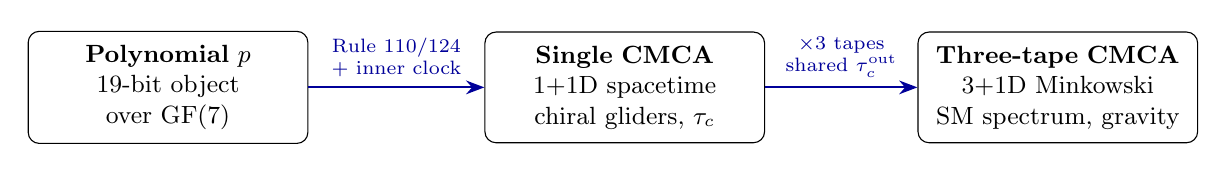
\begin{tikzpicture}[
  box/.style={draw,rounded corners,fill=white,text width=3.2cm,align=center,
    font=\small,inner sep=5pt},
  arr/.style={-{Stealth},thick,blue!60!black}
]
\node[box] (poly) at (0,0)
  {\textbf{Polynomial $p$}\\ 19-bit object\\over GF(7)};
\node[box] (cmca) at (5.8,0)
  {\textbf{Single CMCA}\\ 1+1D spacetime\\chiral gliders, $\tau_c$};
\node[box] (three) at (11.3,0)
  {\textbf{Three-tape CMCA}\\ 3+1D Minkowski\\SM spectrum, gravity};
\draw[arr] (poly.east) -- node[above,font=\scriptsize,align=center]{Rule~110/124\\+ inner clock} (cmca.west);
\draw[arr] (cmca.east) -- node[above,font=\scriptsize,align=center]{$\times 3$ tapes\\shared $\tau_c^{\rm out}$} (three.west);
\end{tikzpicture}
\end{center}
\vspace{4pt}
\small Every arrow is a theorem, not an assumption.  The
shared clock (rightmost step) is necessary and sufficient by the DPP (\CatAL).
The continuum limit gives the $\Phi_{\rm MDL}$ field and General Relativity.
\end{tcolorbox}

\subsection{Falsifiable predictions}

The three-tape construction makes two zero-parameter predictions that
distinguish it from alternatives:
\begin{itemize}
  \item \textbf{Tensor-to-scalar ratio:} $r = 0$ (no primordial gravitational
        waves from the three-tape vacuum).
  \item \textbf{CP-violation phase:} $\delta_{CP} = 205.71^\circ$
        (from the $\mathbb{Z}_7$ winding structure; PMNS matrix prediction).
\end{itemize}

%─────────────────────────────────────────────────────────────────────────────
\section{Summary and Quick Reference}
\label{sec:summary}
%─────────────────────────────────────────────────────────────────────────────

\begin{tcolorbox}[colback=boxblue,colframe=blue!50!black,
  title=The three-tape CMCA in one paragraph]
Take the GTE polynomial $p(L,C,R) = C + R - CR - LCR$ over $\mathrm{GF}(7)$.
Run it on three 1D tapes simultaneously, synchronized by a single shared
clock $\tau_c^{\rm out}$.  Each tape represents one spatial dimension; the
shared clock is time.  The right-chiral layer of each tape uses Rule~110;
the left-chiral layer uses Rule~124 (its mirror image).  By the Dimensional
Protocol Principle (DPP, machine-certified), this construction is the unique
minimal mechanism that gives 3+1D Minkowski dynamics.  The inner clock fires
at $3/7$ the rate of the outer clock, implementing Lorentz time dilation.
The Lorentz algebra, baryon number, color confinement, parity violation, and
quantum entanglement all follow from the same 19-bit polynomial.
\end{tcolorbox}

\bigskip
\noindent\textbf{Key Lean certifications (all zero sorry):}

\begin{center}
{\small
\begin{tabular}{P{4.5cm}P{5.5cm}P{2.0cm}}
\toprule
What is proved & Lean theorem name & Status \\
\midrule
Shared clock needed for 3+1D &
  \lean{dimensional\_protocol\_principle\_master} & \CatAL \\[4pt]
Tensor product gives $\mathbb{R}^{3,1}$ &
  \lean{cmca\_tensor\_product\_gives\_31d\_minkowski} & \CatAL \\[4pt]
All 12 Lorentz algebra relations &
  \lean{lorentz\_algebra\_complete} & \CatAL \\[4pt]
Rule~124 = Rule~110 reflected &
  \lean{rule124\_eq\_rule110\_reflected} & \CatAL \\[4pt]
No finite CA gives exact Lorentz &
  \lean{no\_finite\_ca\_exact\_lorentz\_replica} & \CatAL \\[4pt]
Causal diamond $V(T) = T^4/4$ &
  \lean{three\_tape\_causal\_diamond\_t4} & \CatAL \\[4pt]
Holographic ratio $\to 0$ &
  \lean{holographic\_ratio\_vanishes} & \CatAL \\[4pt]
Vacuum is Ricci-flat &
  \lean{three\_tape\_gorard\_vacuum\_ricci\_flat} & \CatAL \\[4pt]
SR time dilation $\tau_c/T = 3/7$ &
  \lean{sr\_ratio\_measurement.py} (numerical) & \CatA \\
\bottomrule
\end{tabular}
}
\end{center}

\bigskip
\noindent\textbf{Where to go next:}
\begin{itemize}
  \item P41 (\href{https://novaspivack.com/research}{novaspivack.com/research}):
        the single-tape CMCA and its 1+1D dynamics.
  \item P45 (\href{https://doi.org/10.5281/zenodo.20465805}{doi.org/10.5281/zenodo.20465805}):
        the three-tape construction, DPP proof, and all results in this tutorial.
  \item P42--P43: the $\Phi_{\rm MDL}$ continuum field and its completeness theorem
        (Level~2 physical substrate).
  \item P48~\cite{SpivackGTECompleteFramework} monograph
        (\href{https://doi.org/10.5281/zenodo.20560550}{doi.org/10.5281/zenodo.20560550}):
        the full GTE framework, incorporating the three-tape architecture and all
        downstream physics.
  \item \texttt{ugp-lean} repository
        (\href{https://github.com/novaspivack/ugp-lean}{github.com/novaspivack/ugp-lean}):
        all Lean 4 proofs, zero sorry, zero custom axioms.
\end{itemize}


\section*{Further Reading}
\begin{tcolorbox}[colback=orange!8,colframe=orange!50!black,
  title=\textbf{Primary Sources}]
The results in this tutorial are derived in the following papers,
all available open-access on Zenodo and at
\href{https://novaspivack.com/research}{novaspivack.com/research}:
\begin{itemize}
  \item \textbf{P41 --- The Three-Layer Chiral Minkowski CA} (single-tape architecture):\\
        \href{https://doi.org/10.5281/zenodo.20417572}{doi.org/10.5281/zenodo.20417572}
  \item \textbf{P45 --- The Three-Tape CMCA} (DPP, 3+1D emergence, all theorems):\\
        \href{https://doi.org/10.5281/zenodo.20465805}{doi.org/10.5281/zenodo.20465805}
  \item \textbf{P48 --- The Complete GTE Framework} (main synthesis monograph):\\
        \href{https://doi.org/10.5281/zenodo.20560550}{doi.org/10.5281/zenodo.20560550}
\end{itemize}
Lean~4 machine proofs: \href{https://github.com/novaspivack/ugp-lean}{github.com/novaspivack/ugp-lean}
\end{tcolorbox}

\bibliography{../../papers/bib/Spivack_Papers_Bibliography}
\end{document}
